\section{Introduction}

This paper describes the software framework, tools, and algorithms that were developed in support of event
reconstruction and analysis of the CLAS12 (CEBAF Large Acceptance Spectrometer at 12 GeV) experiment at
Jefferson Lab (JLab)~\cite{clas12-nim}. Installed in experimental Hall~B, CLAS12 is a large acceptance
spectrometer based on two superconducting magnets and multiple detector subsystems that provides large
coverage for the detection of charged and neutral particles produced by the interaction of the electron beam
from the JLab CEBAF accelerator with a target located at the center of the spectrometer. A six-coil torus
magnet defines the six-sector structure of the so-called Forward Detector that is outfitted with Drift
Chambers~\cite{dc-nim} for charged particle tracking and multiple detector systems for particle identification.
These detectors include threshold Cherenkov Counters~\cite{ltcc-nim,htcc-nim} and Ring-Imaging Cherenkov
Counters~\cite{rich-nim}, scintillator-based time-of-flight hodoscopes~\cite{ftof-nim}, and electromagnetic
calorimeters~\cite{ecal-nim}. In the target region, a 5~T superconducting solenoid surrounds a central tracker
based on silicon and Micromegas detectors \cite{svt-nim,mm-nim}, and subsystems for particle identification
that include a time-of-flight scintillation counter barrel~\cite{ctof-nim} and a neutron detector~\cite{cnd-nim},
forming the so-called Central Detector.

Figure~\ref{clas12-model} shows a model representation of the CLAS12 spectrometer identifying the Forward
and Central Detectors. In between the central and forward region, the CLAS12 Forward Tagger~\cite{ft-nim}
extends the kinematic coverage for the detection of electrons and photons at polar angles from 2$^\circ$ to
5$^\circ$. Figure~\ref{ft-model} shows a model representation of the Forward Tagger. The total number of
readout channels of CLAS12 is larger than 100k. Typical trigger rates are 15 kHz. In 2018, data rates of
500~MB/s with a live time of $>$ 95\% were achieved.

\begin{figure}[t]
\centering
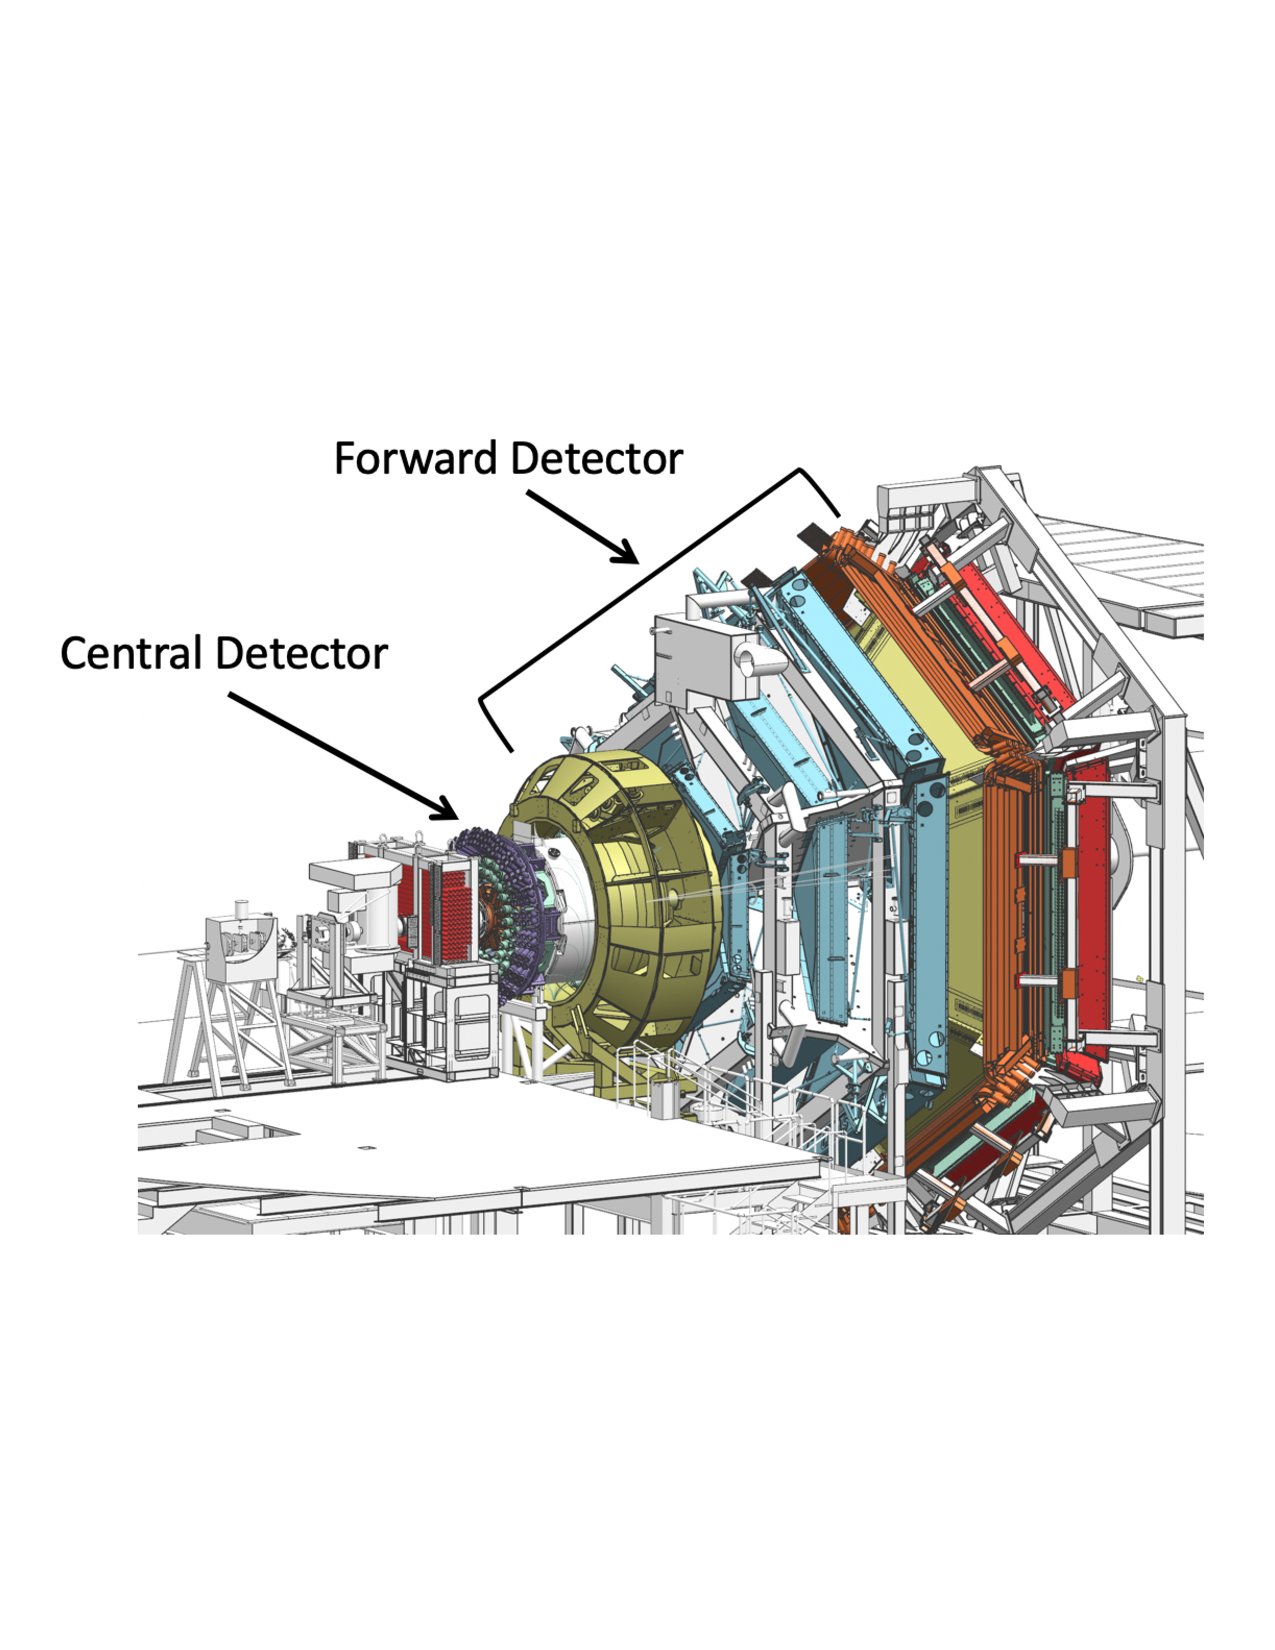
\includegraphics[width=0.48\textwidth]{pics/clas12-model.pdf}
\caption{Model representation of the CLAS12 spectrometer in Hall~B at Jefferson Laboratory. The electron
  beam is incident from the left side of this figure. The CLAS12 detector is roughly 20~m in scale along the
  beam axis. The CLAS12 Forward and Central Detectors are identified.}
\label{clas12-model}
\end{figure}

\begin{figure}
\centering
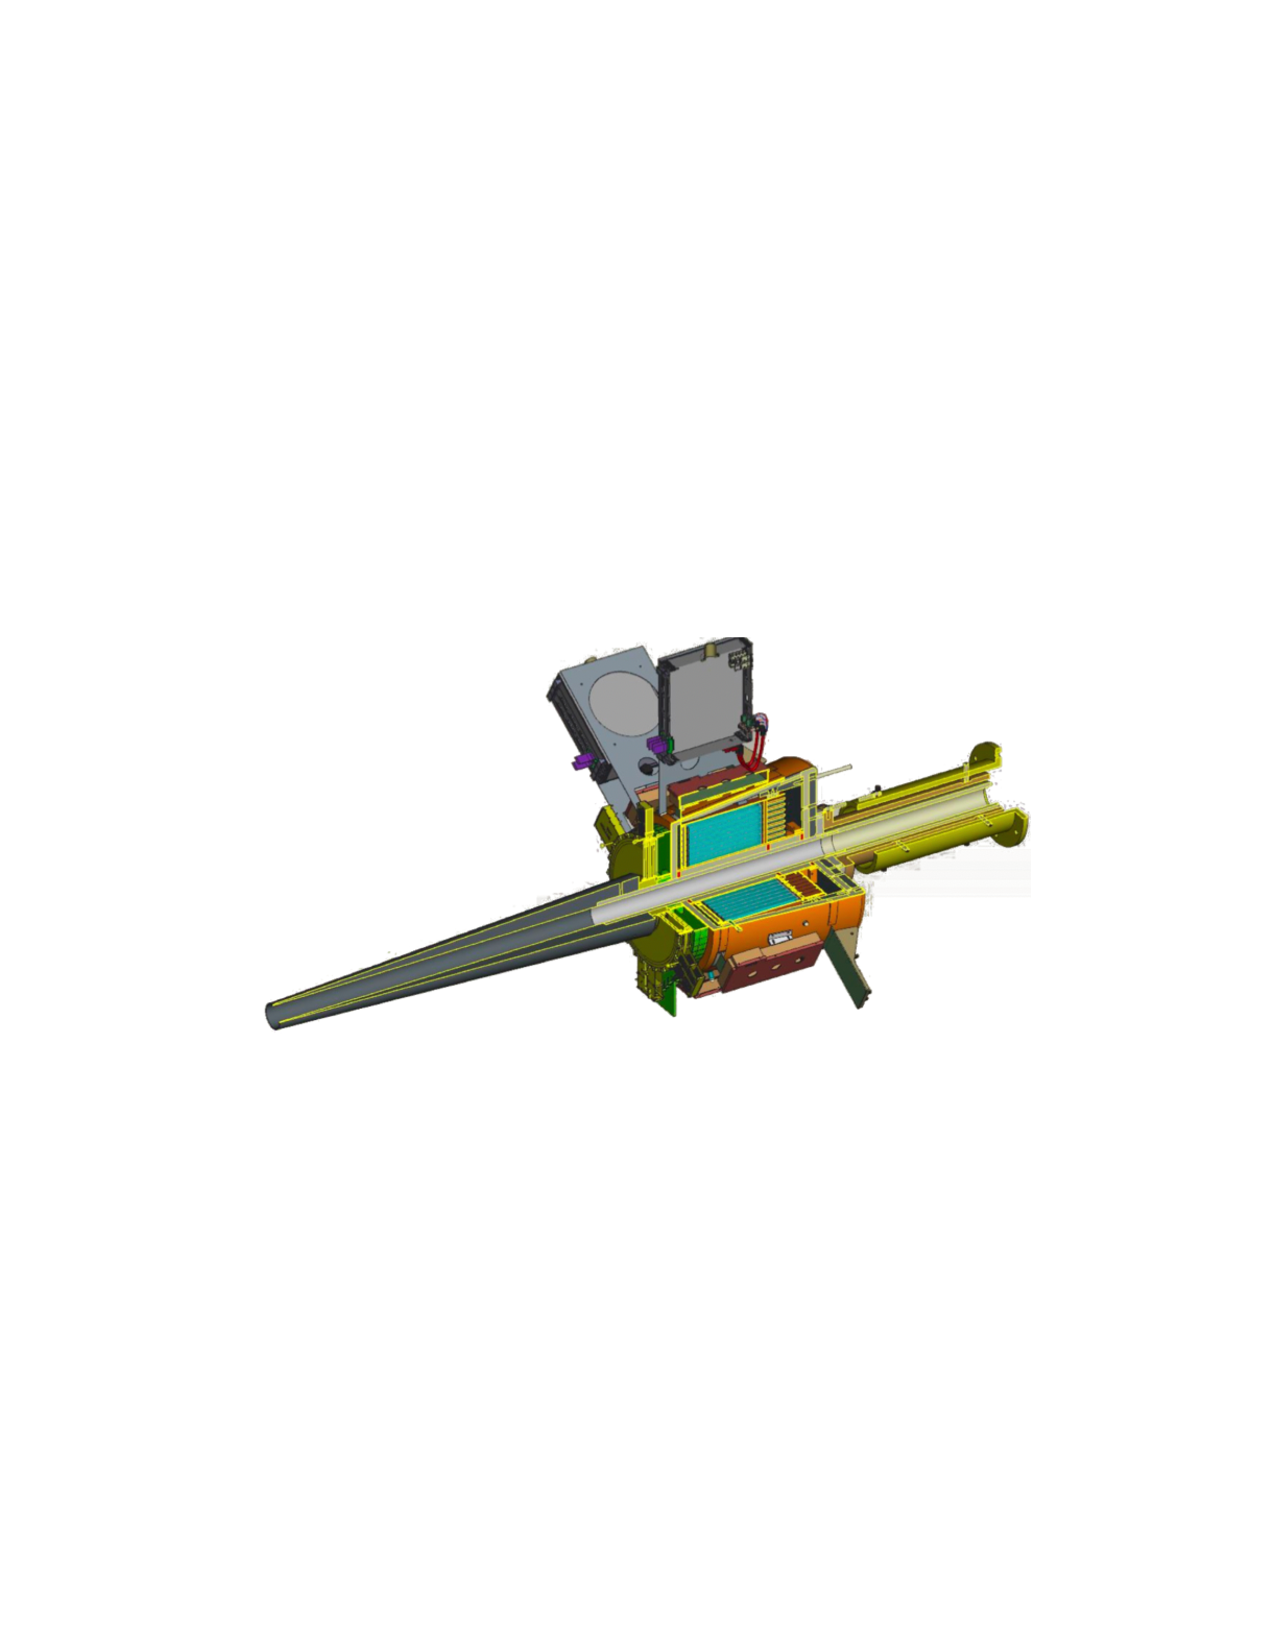
\includegraphics[width=0.48\textwidth]{pics/ft-model.pdf}
\caption{Model representation in a cut view of the CLAS12 Forward Tagger that is positioned just upstream of
  the torus magnet along the beam axis. Attached to the upstream face of the detector is the M{\o}ller electron
  shielding cone.}
\label{ft-model}
\end{figure}

The CLAS12 offline reconstruction and analysis framework was developed to cope with the complexity of the
spectrometer and the related data volumes. It consists of an extensive library of software tools, of detector
reconstruction packages, and a framework to chain the reconstruction and analysis applications for data
processing. Software tools have been designed to support and standardize event reconstruction, detector
calibration and monitoring, and data analysis, providing I/O functionalities, database access, detector geometry
libraries, and tools to handle magnetic fields. These constitute the building blocks for the development of all
CLAS12 detector monitoring, calibration, and reconstruction tools. Each reconstruction package is designed to
extract from the raw data the relevant information for particle reconstruction, such as tracks, hits, or clusters.
These are the input information for the CLAS12 Event Builder, which sifts through the reconstructed detector
output to identify particles and form the reconstructed event. The reconstruction components are deployed in a
service-oriented platform, which provides the functionalities for data processing for both event reconstruction
and the subsequent analysis. While the software framework supports multiple programming languages, the CLAS12
reconstruction packages and tools currently in use are developed in Java.

This paper is organized as follows. The CLAS12 software framework and tools are described in
Section~\ref{sec:framework}. The raw and reconstructed data formats are presented in Section~\ref{sec-formats}.
The monitoring, calibration, and event display applications are described in Sections~\ref{sec:calibration} and
\ref{sec:ced}. Section~\ref{sec:recon} provides a detailed description of the detector and event reconstruction
packages, including selected results from reconstruction of simulated data that have been used to develop and
validate the algorithms. The reconstruction performance on beam data is presented in Ref.~\cite{clas12-nim}.
Finally, Sections~\ref{sec:dataproc} and \ref{sec:manage} present the data processing and code management
procedures adopted for CLAS12.
